% Chapitre de contribution n° 2 (TOP20 pick 2, id Z-BAO-P23)
% Sources : papers/certified_desi_h0/ (certified_desi_h0.tex, publication_meta.json),
% results/certified_numerics/P2_likelihood/ et P3_h0/ (result.json, verification.md), TOP20.json.
\chapter[Une tension écrite comme une inégalité]{Une tension célèbre de la cosmologie, écrite comme une inégalité vérifiée}
\reference{Publié le 10 octobre 2026.\\ doi:10.5281/\\zenodo.23284020}

\section*{L'idée en une image}

\begin{analogie}
Imaginez qu'on veuille prouver qu'une radio ne capte aucune station au-delà de la graduation 73. On ne peut pas
écouter une infinité de positions du bouton. Alors on découpe le cadran en bandes, et pour chaque bande un notaire
signe une attestation : « dans toute cette bande, le signal reste sous tel niveau ». Quand toutes les bandes sont
signées, le cadran entier est couvert, sans trou.

\emph{Où l'image s'arrête :} ici, « pas de station » veut dire « les données s'ajustent bien plus mal », pas
« c'est impossible » ; et l'attestation ne vaut que pour la radio qu'on a décrite, c'est-à-dire pour le modèle choisi.
\end{analogie}

\section*{Ce qui a été fait}

L'univers s'étend, et son taux d'expansion actuel s'appelle $H_0$. Deux familles de mesures ne s'accordent pas sur sa
valeur : c'est la « tension de Hubble ». Les mesures proches, par une échelle de distances, se situent vers
73\,km/s par mégaparsec. Les mesures de la règle standard du chapitre précédent, combinées avec ce que les premières
minutes de l'univers nous disent sur les éléments légers, donnent environ 68,5 (DESI publie $68{,}51\pm0{,}58$).

Le travail transforme deux affirmations connues en théorèmes contrôlés par la machine. La première : avec les seules
mesures de DESI, une part de matière $\Omega_m$ entre 0 et 0,255 ou entre 0,35 et 1 s'ajuste beaucoup plus mal que
le meilleur ajustement, quelle que soit la taille de la règle. La seconde : avec en plus les éléments légers, toute
valeur $H_0\ge73$ s'ajuste beaucoup plus mal, quels que soient la part de matière et la densité de baryons. « Beaucoup
plus mal » a un sens précis : un score d'écart, noté $\chi^2$, dépasse de plus de 25 celui d'un point de référence
certifié ($\chi^2\le10{,}2897$).

\begin{encadre}
\textbf{À faire avec un crayon : couvrir une infinité de valeurs d'un seul coup.} La taille de la règle est une
inconnue $t$ qui peut prendre n'importe quelle valeur. Le score a la forme $c-Bt+At^2$. Prenons $3-2t+t^2$. On le
réécrit $(t-1)^2+2$ : un carré n'est jamais négatif, donc le score vaut au moins $2$ \emph{pour tout} $t$.
Vérifiez : $t=0$ donne $3$, $t=1$ donne $2$, $t=3$ donne $6$. En général, si $A>0$, le score vaut au moins
$c-B^2/(4A)$ ; ici $3-4/4=2$. Une seule inégalité règle une infinité de cas.

\textbf{Le seuil.} $35{,}2897-10{,}2897=25=5^2$ : c'est l'écart conventionnel appelé « 5 sigmas » quand on
s'intéresse à un seul paramètre (environ 4,3 sigmas si on lit la région jointe des trois paramètres).
\end{encadre}

Pour couvrir toutes les valeurs des paramètres, l'espace est découpé en tranches et en boîtes, comme le cadran de la
radio : 29 tranches pour la part de matière, 89 boîtes pour la question de $H_0$. Sur chaque boîte, un évaluateur
d'intervalles, prouvé correct une fois pour toutes, borne le score par des fractions exactes. La
figure~\ref{fig:c02} montre la même chose calculée de façon ordinaire : la courbe franchit le seuil 25 vers
$H_0\approx71{,}6$, et l'écart au meilleur point vaut environ $54{,}6$ à $H_0=73$. La valeur 73 est donc une valeur de référence, choisie
d'avance ; ce n'est pas le bord de la région exclue.

\begin{figure}[htbp]
\centering
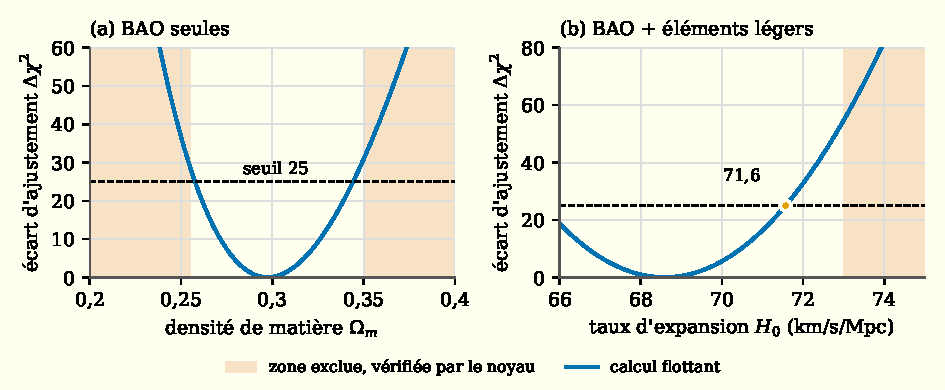
\includegraphics[width=\linewidth]{figures/c02_profils}
\caption{Courbes : calcul flottant ordinaire recalculé à partir des données (niveau X). Zones ombrées : ce que le
noyau a vérifié. (a) Part de matière, DESI seul. (b) Taux d'expansion, DESI et éléments légers.}
\label{fig:c02}
\end{figure}

\section*{Comment on s'est assuré que ce n'est pas faux}

\niveau{As} \emph{Le juge a regardé, sans rejeu.} Le juge est Lean, un programme qui contrôle chaque pas d'une preuve.
Les bornes de logarithmes et d'exponentielles viennent de résultats déjà prouvés dans sa bibliothèque mathématique,
et seules les trois hypothèses de base admises partout apparaissent. Ces fichiers ne figurent pas dans le rejeu complet
du 26 octobre : d'où « sans rejeu ».

Les tests faits pour échouer ont échoué. Une copie des données dont une valeur est décalée de 10 écarts-types fait
bondir le score certifié vers $[122{,}69\,;\,122{,}76]$. Une tranche qui contient le meilleur ajustement n'est pas
exclue. Surtout, un vérificateur indépendant a reconstruit les 173 modules du théorème final et constaté que la preuve
casse si l'on demande un seuil de 65 au lieu de $35{,}29$ : c'est normal, car l'énoncé deviendrait faux (le score vaut
$64{,}91$ à $H_0=73$).

Un échec a aussi été publié. Le découpage en tranches fixé \emph{avant} le calcul n'a exclu que 8 tranches sur 19 ;
la prédiction annoncée n'était pas tenue. Un découpage plus fin, décidé après coup, a été déclaré comme tel. Deux
vérifications indépendantes par des agents d'IA (dont la reconstruction de 3 des 29 tranches) ont donné un avis
favorable avec corrections. Aucun humain n'a refait ces calculs.

\section*{Ce que ça ne dit pas}

\begin{limite}
\begin{itemize}
\item C'est une version certifiée d'une tension déjà connue par les statistiques ordinaires, pas une nouvelle mesure.
\item Le modèle est simplifié : univers plat, rayonnement négligé, une formule d'ajustement pour la taille de la
règle, des erreurs supposées gaussiennes.
\item Rien ici ne dit d'où vient la tension, ni laquelle des deux familles de mesures a raison.
\item Le côté bas ($H_0\le64$), prévu comme secondaire, n'a pas été tenté.
\end{itemize}
\end{limite}

\section*{Pour aller plus loin}

Le même travail montre aussi qu'un univers fait uniquement de matière s'ajuste très mal à ces données (score au moins
$1415{,}82$, quelle que soit la règle). Article et fichiers : doi:10.5281/zenodo.23284020.
